\documentclass[12pt, a4paper, oneside]{article}
\usepackage[T1]{fontenc}
\usepackage{amsmath, amsthm, amssymb, bm, color, enumitem, graphicx, hyperref, mathrsfs, titling}
\usepackage[UTF8, scheme = plain]{ctex}
\usepackage{graphicx, minted, listings}
\title{\textbf{Homework 1}}
\setlength{\droptitle}{-10em}
\author{PENG Qiheng \\ Student ID\: 225040065}
\date{\today}
\linespread{1.5}
\newcounter{problemname}
\newenvironment{problem}{\stepcounter{problemname}\par\noindent{Problem \arabic{problemname}. }}{\par}
\newenvironment{solution}{\par\noindent{Solution. }}{\par}

\begin{document}

\maketitle

\begin{problem}
\begin{enumerate}[label = (\alph*)]
    \item In supervised learning, we have a dataset of input data and labels, and the goal is to learn a mapping from inputs to labels.
        \newline In unsupervised learning, we only have input data and the goal is to discover the hidden patterns or structures in the data.
    \item Answer: 2
        \newline 1. Regression is used to fit continuous labels.
        \newline 3. For a given training dataset, perceptrons with different initialization may converge to different linear classifiers.
        \newline 4. Least squares is a maximum likelihood estimator only if error follows a Gaussian Distribution.
    \item 1. Since we have
        \begin{equation} r(\bm{X}^T\bm{X}) = r(\bm{X}) = d \end{equation}
        \begin{equation}\bm{X}^T\bm{X} \in \mathbb{R}^{d \times d} \end{equation}
        thus, $\bm{X}^T\bm{X}$ is invertible
        \newline 2. As
        \begin{equation} {(\bm{X}^T\bm{X})}^T = \bm{X}^T\bm{X} \end{equation}
        we know that $\bm{X}^T\bm{X}$ is Symmetric Matrices
        \newline 3. Thus, we can conclude that $\bm{X}^T\bm{X}$ is Positive Definite
\end{enumerate}
\end{problem}

\newpage
\begin{problem}
\begin{enumerate}[label = (\alph*)]
    \item  Let $\bm X = \bm V \bm \Sigma_1 \bm U_1^T$, $\bm z = \bm U_1^T \bm \theta$ and $\bm A := \bm V \bm \Sigma_1$ we have
        \begin{equation} \min_{\bm \theta \in \mathbb R^d}||\bm X\bm \theta - \bm y||_2^2 = \min_{\bm \theta \in \mathbb R^d}||\bm V \bm \Sigma_1 \bm U_1^T \bm \theta - \bm y||_2^2 = \min_{\bm z \in \mathbb R^n}||\bm A \bm z - \bm y||_2^2 \end{equation}
        Since $\bm A$ is of full rank, we have optimal $\bm z$
        \begin{equation} \bm z^* = \bm A^{-1} \bm y \end{equation}
        And we have
        \begin{equation} \bm U_1^T\bm \theta^* = \bm A^{-1} \bm y \end{equation}
        \begin{equation} \bm U_1^T\bm \theta^* - \bm A^{-1} \bm y = \bm 0 \end{equation}
        Considering that $\bm U^T_1 \bm U_2 = \bm 0$
        \begin{equation} \bm U_1^T\bm \theta^* - \bm A^{-1} \bm y = \bm U^T_1 \bm U_2 \end{equation}
        \begin{equation} \bm \theta^* = \bm U_1 {(\bm V \bm \Sigma_1)}^{-1} \bm y + \bm U_2 \bm c, \bm c \in \mathbb R^{d-n} \end{equation}
        And the optimal function value is $0$, if $\bm c = \bm 0$
    \item Let
        \begin{equation} \mathcal L(\bm \theta) = ||\bm X\bm \theta - \bm y||_2^2 + \lambda ||\bm \theta||_2^2 \end{equation}
        Take the gradient
        \begin{equation} \nabla \mathcal L(\bm \theta) = 2\bm X^T(\bm X\bm \theta - \bm y) + 2\lambda \bm \theta \end{equation}
        \begin{equation} (\bm X^T \bm X + \lambda \bm I) \bm \theta^* = \bm X^T \bm y \end{equation} 
        Since $\bm X^T \bm X$ is semi-positive definite and $\bm X^T \bm X + \lambda \bm I$ is positive definite. Thus, we have
        \begin{equation} \bm \theta^* = {(\bm X^T \bm X + \lambda \bm I)}^{-1} \bm X^T \bm y \end{equation} 
\end{enumerate}
\end{problem}

\newpage
\begin{problem}
\begin{enumerate}[label = (\alph*)]
    \item As the assumption, we have
        \begin{equation} \epsilon_i = y_i - \bm X_i \bm \theta \end{equation}
        \begin{equation} P(D|\bm \theta) = \Pi_{i=1}^n (\frac{1}{2b} e^{-\frac{|y_i - \bm X_i \bm \theta|}{b}}) = {2b}^{-n} e^{-\frac{{|\bm y - \bm X \bm \theta|}}{b}} \end{equation}
        Let $\mathcal L(\bm \theta) = \log{P(D|\bm \theta)}$, we have
        \begin{equation} \mathcal L(\bm \theta) = -n\log{(2b)} - \frac{1}{b}{|\bm y - \bm X \bm \theta|} \end{equation}
        \begin{equation} \bm \theta^* = \arg\max_{\bm \theta} \mathcal L(\bm \theta) = \arg\min_{\bm \theta} {|\bm y - \bm X \bm \theta|} \end{equation}
    \item According to the definition of $h_\mu(z)$, we have
        \begin{equation} \frac{\partial h_\mu(z)}{\partial z} = \begin{cases} sign(z), & |z| \ge \mu \\
        \frac{z}{\mu}, & |z| \le \mu \end{cases} \end{equation}
        And we can rewrite $h'_\mu(z)$ as
        \begin{equation} h'_\mu(z) = \frac{z}{\max(|z|, \mu)} \end{equation}
        Thus, we have
        \begin{equation} H'_\mu(\bm z) = \frac{\partial \Sigma_{j=1}^n h_\mu(z_j)}{\partial \bm z} = \begin{bmatrix} h'_\mu(z_1) \\ \vdots \\ h'_\mu(z_n) \end{bmatrix} = h'_\mu(\bm z) \end{equation}
        Finally, we have
        \begin{equation} \nabla \mathcal L(\bm\theta) = \frac{\partial (\bm X \bm \theta - \bm y)}{\partial \bm \theta} \frac{\partial H_\mu(\bm z)}{\partial \bm z} = \bm X^T h'_\mu (\bm X \bm \theta - \bm y) \end{equation}
    \item \quad \\
        After calculating, output $||\bm\hat\theta_{LS} - \bm\theta^*|| = 59.5136$ \\
        code as follows:
        \begin{lstlisting}[language=Python, basicstyle=\small, numbers=left, stepnumber=1, numbersep=5pt, columns=fullflexible, keepspaces=true, lineskip=0.1em]
        import numpy as np
        import matplotlib.pyplot as plt
        d = 50  # feature dimension
        X = np.load("data/X.npy")
        y = np.load("data/y.npy")
        print("data shape: ", X.shape, y.shape)
        theta_star = np.load("data/theta_star.npy")
        ###### part (1): least square estimator ########
        theta_hat = np.linalg.inv(X.T @ X) @ X.T @ y
        Error_LS = np.linalg.norm(theta_hat - theta_star, 2)
        print("Estimator approximated by LS:", Error_LS)
        ###### part (2): L1 estimator ########
        mu = 1e-5  # smoothing parameter
        alpha = 0.001  # stepsize
        T = 1000  # iteration number
        # random initialization
        theta = np.random.randn(d, 1)
        Error_huber = []
        for _ in range(1, T):
            # calculate the l2 error of the current iteration
            Error_huber.append(np.linalg.norm(theta - theta_star, 2))
            # calculate gradient
            z = X @ theta - y
            h_prime = z / np.maximum(np.abs(z), mu)
            grad = X.T @ h_prime
            # gradient descent update
            theta = theta - alpha * grad
        #######   plot the figure   #########
        plt.figure(figsize=(10, 5))
        plt.yscale("log", base=2)
        plt.plot(Error_huber, "r-")
        plt.title(r"$\ell_1$ estimator approximated by Huber")
        plt.ylabel(r"$\theta$")  # set the label for the y axis
        plt.xlabel("Iteration")  # set the label for the x axis
        plt.show()
        \end{lstlisting}
        The Huber smoothing error is shown in Figure 1.
        \begin{figure}[htbp]
            \centering
            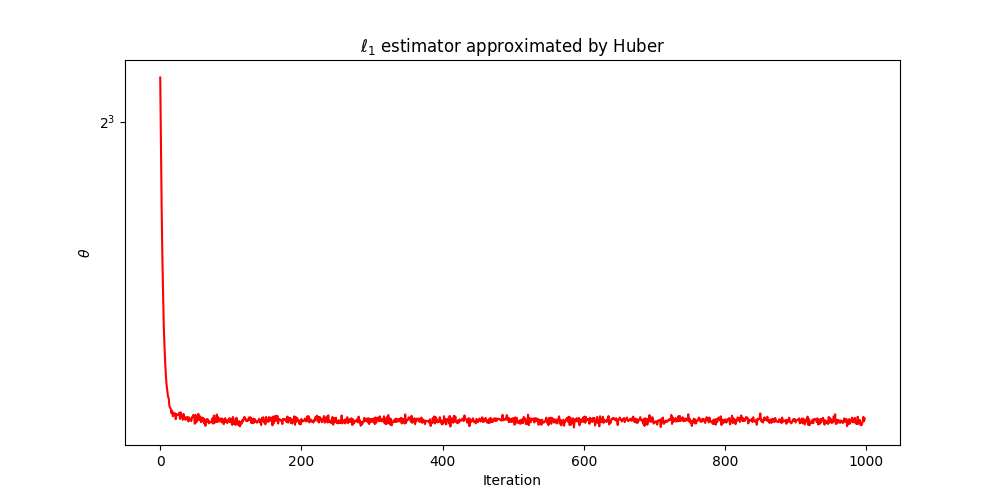
\includegraphics[width=1\textwidth]{../code_source/p3/theta_error.png}
            \caption{Huber smoothing error}
        \end{figure}
\end{enumerate}
\end{problem}

\newpage
\begin{problem}
\begin{enumerate}[label = (\alph*)]
    \item Since $\theta^*$ is a classifier that correctly separates all the data points, we can get
        \begin{equation} \notag y_i({\bm\theta^*}^T \bm x_i) > 0, \forall i = 1, \ldots, n \end{equation}
        We can easily have
        \begin{equation} \notag \rho \ge y_i({\bm\theta^*}^T \bm x_i) > 0 \end{equation}
    \item According to update (1), we have
        \begin{equation} \notag \bm\theta_k^T\theta^* = \bm\theta_{k-1}^T\theta^* + y_{k-1}\bm x_{k-1}^T\bm\theta^* \ge \bm\theta_{k-1}^T\theta^* + \rho \end{equation}
        After recursion, we have
        \begin{equation} \notag \bm\theta_k^T\theta^* \ge k\rho \end{equation}
    \item According to update (1), we have
        \begin{align} \notag ||\bm\theta_k||^2 &= ||\theta_{k-1} + y_{k-1}\bm x_{k-1}^T||^2 \\
            \notag &= ||\bm\theta_{k-1}||^2 + ||\bm x_{k-1}||^2 + 2y_{k-1}\bm\theta_{k-1}^T\bm x_{k-1} \end{align}
        Since $\bm x_{k-1}$ is misclassified by $\bm\theta_{k-1}$, we have $y_{k-1}\bm\theta_{k-1}^T\bm x_{k-1} \le 0$
        \begin{align} \notag ||\bm\theta_k||^2 \le ||\bm\theta_{k-1}||^2 + ||\bm x_{k-1}||^2 \end{align}
    \item According to the problem, we have $R \ge ||\bm x_i||, \forall i = 1, \ldots, n$
        And we have
        \begin{align} \notag ||\bm\theta_k||^2 \le ||\bm\theta_{k-1}||^2 + ||x_{k-1}||^2 \le ||\bm\theta_{k-1}||^2 + R^2 \end{align}
        After recursion, we have
        \begin{align} \notag ||\bm\theta_k||^2 \le kR^2 \end{align}
    \item According to steps 2 and 4, we have $\bm\theta_k^T\bm\theta^* \ge k\rho$ and $||\bm\theta_k||^2 \le kR^2$
        we can get
        \begin{align} \notag \frac{\bm\theta_k^T\bm\theta^*}{||\bm\theta_k||} \ge \sqrt{k}\frac{\rho}{R} \end{align}
        By using Cauchy-Schwarz inequality, we have
        \begin{align} \notag k^2\rho^2 \le ||\bm\theta_k||^2||\bm\theta^*||^2 \le kR^2||\theta^*||^2 \end{align}
        Thus, we have
        \begin{align} \notag \bar k \le \frac{R^2||\theta^*||^2}{\rho^2} \end{align}
\end{enumerate}
\end{problem}


\newpage
\begin{problem}
    Main code as follows:
        \begin{lstlisting}[language=Python, basicstyle=\small, numbers=left, stepnumber=1, numbersep=5pt, columns=fullflexible, keepspaces=true, lineskip=0.1em]
        # train
        iters = 2000
        d = 2
        num_sample = X.shape[0]
        threshold = 1e-4
        theta = np.zeros((d + 1, 1))
                
        X = np.hstack([X, np.ones((num_sample, 1))])
        X_test = np.hstack([X_test, np.ones((X_test.shape[0], 1))])
        Er_in_perceptron = []
        Er_out_perceptron = []
        Er_in_pocket = []
        Er_out_pocket = []
        pocket = theta.copy()
        best_error = cal_error(theta, X, y)
                
        for iterate in range(iters):
            for i in random.sample(range(num_sample), num_sample):
                if np.sign(X[i] @ theta)[0] != y[i]:
                    theta += (y[i] * X[i]).reshape(-1, 1)
                    break
                
            cur_error = cal_error(theta, X, y)
            if cur_error < best_error:
                best_error = cur_error
                pocket = theta.copy()
                
            Er_in_perceptron.append(cur_error)
            Er_out_perceptron.append(cal_error(theta, X_test, y_test))
            Er_in_pocket.append(best_error)
            Er_out_pocket.append(cal_error(pocket, X_test, y_test))
                
        # print(f"theta (perceptron): {theta}")
        # print(f"pocket (pocket): {pocket}")
                
        # plot Er_in and Er_out
        fig, axs = plt.subplots(1, 2, figsize=(14, 6))
                
        # perceptron
        axs[0].plot(Er_in_perceptron, label="Perceptron Train Error")
        axs[0].plot(Er_in_pocket, label="Pocket Train Error")
        axs[0].set_xlabel("Iteration")
        axs[0].set_ylabel("Error Rate")
        axs[0].set_title("Training Error")
        axs[0].legend()
        # pocket
        axs[1].plot(Er_out_perceptron, label="Perceptron Test Error")
        axs[1].plot(Er_out_pocket, label="Pocket Test Error")
        axs[1].set_xlabel("Iteration")
        axs[1].set_ylabel("Error Rate")
        axs[1].set_title("Test Error")
        axs[1].legend()
                
        plt.tight_layout()
        plt.show()
                
        # plot decision boundary
        fig, axs = plt.subplots(1, 2, figsize=(14, 6))
                
        ax0 = plot_feature(X, y, plot_num=500, ax=axs[0], classes=np.unique(y))
        x1 = np.linspace(X[:, 0].min(), X[:, 0].max(), 100)
        x2_perceptron = -(theta[0] * x1 + theta[2]) / theta[1]
        x2_pocket = -(pocket[0] * x1 + pocket[2]) / pocket[1]
        ax0.plot(x1, x2_perceptron, "r--", label="Perceptron Boundary")
        ax0.plot(x1, x2_pocket, "b-", label="Pocket Boundary")
        ax0.set_title("Decision Boundaries (Train)")
        ax0.legend()
                
        ax1 = plot_feature(X_test, y_test, plot_num=500, ax=axs[1], classes=np.unique(y_test))
        x1_test = np.linspace(X_test[:, 0].min(), X_test[:, 0].max(), 100)
        x2_perceptron_test = -(theta[0] * x1_test + theta[2]) / theta[1]
        x2_pocket_test = -(pocket[0] * x1_test + pocket[2]) / pocket[1]
        ax1.plot(x1_test, x2_perceptron_test, "r--", label="Perceptron Boundary")
        ax1.plot(x1_test, x2_pocket_test, "b-", label="Pocket Boundary")
        ax1.set_title("Decision Boundaries (Test)")
        ax1.legend()
                
        plt.tight_layout()
        plt.show()
        \end{lstlisting}
        \begin{figure}[htbp]
            \centering
            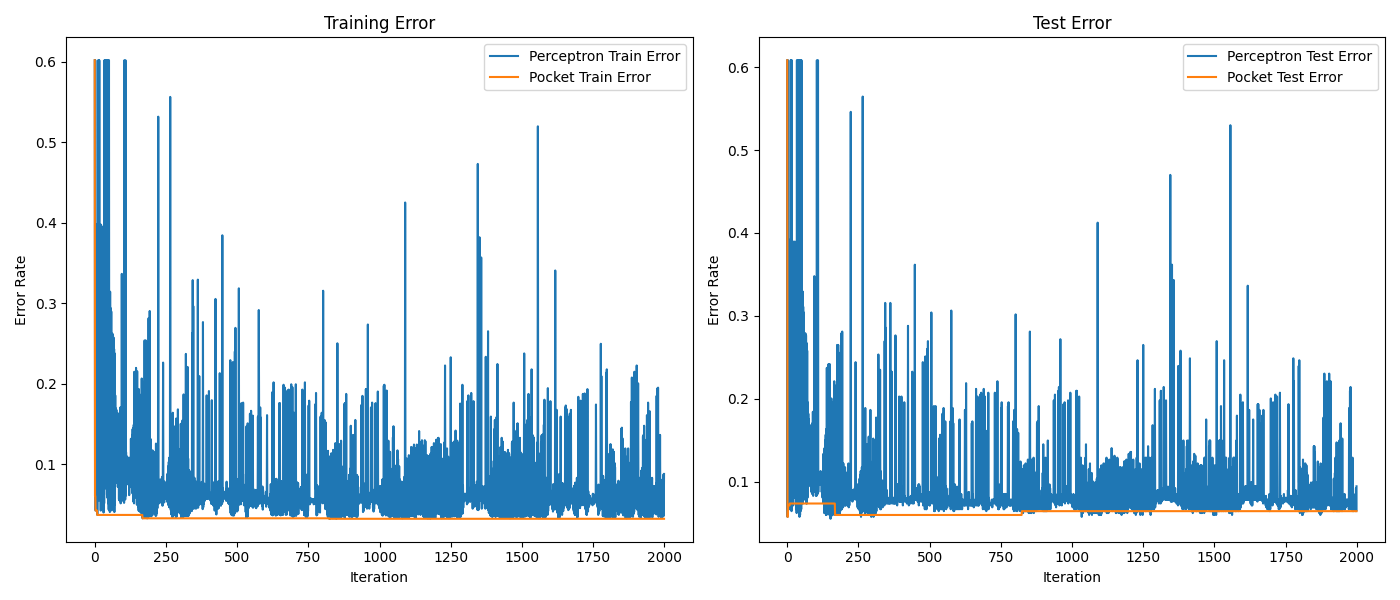
\includegraphics[width=1\textwidth]{../code_source/p5/error_by_iteration.png}
            \caption{Training and Test Error Rate}
        \end{figure}

        From the Figure 2, we observe that:
        \newline The error of the Perceptron algorithm fluctuates more, showing that the Perceptron is sensitive to noisy or non-separable samples.
        \newline The Pocket algorithm maintains and uses the best solution found so far, so its test error curve is smoother and lower than that of the Perceptron. The error of pocket algorithms decreases as the number of iterations increases.
        \newline And the out-of-sample error is generally higher than the in-sample error as we study in lectures.
        \newline Overall, the Pocket algorithm is more robust to outliers and non-separable data.
        \newline The decision boundaries of the two algorithms are shown in Figure 3.
        \begin{figure}[htbp]
            \centering
            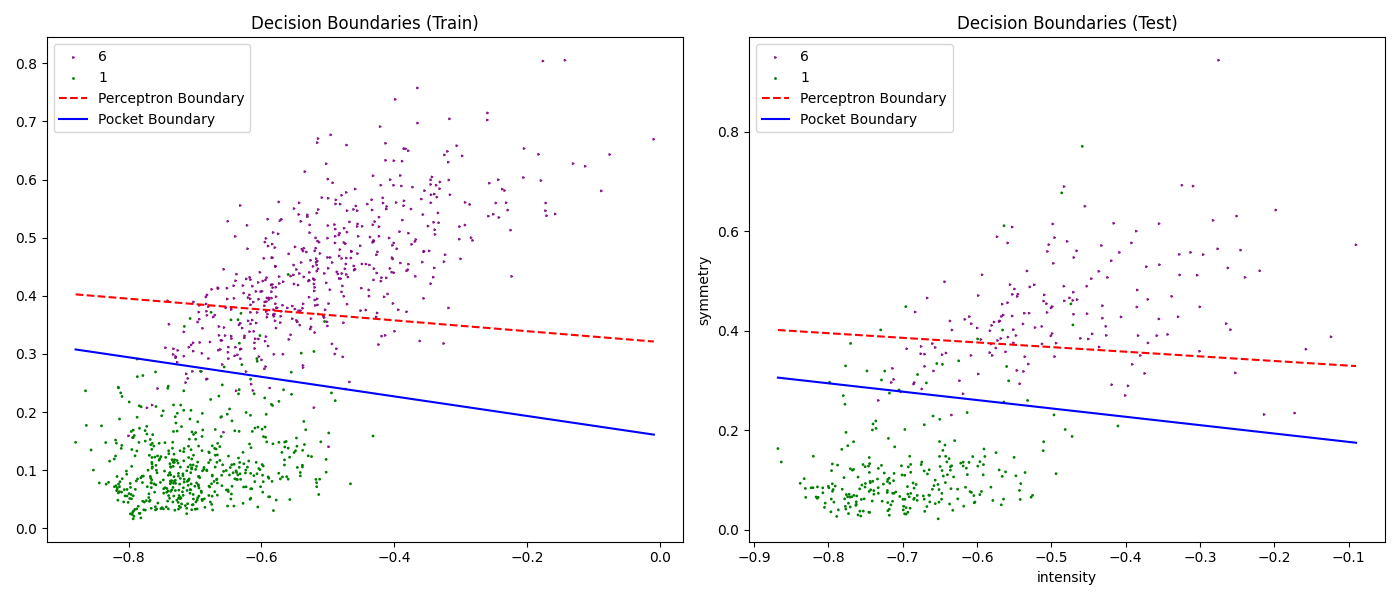
\includegraphics[width=1\textwidth]{../code_source/p5/decision_boundaries.png}
            \caption{Decision Boundaries}
        \end{figure}
\end{problem}

\end{document}